\documentclass[11pt,letterpaper]{article}

\usepackage[margin=1in]{geometry}
\usepackage{graphicx}
\usepackage{subcaption}
\usepackage{booktabs}
\usepackage{hyperref}
\usepackage{parskip}
\usepackage{float}
\usepackage{microtype}
\usepackage{soul}
\usepackage{amsmath}

\hypersetup{colorlinks=true, linkcolor=blue, urlcolor=blue}

\title{\textbf{CS5330 Computer Vision: Project 4}\\
       \large Camera Calibration and Augmented Reality}
\author{Shriman Raghav Srinivasan}
\date{June 2026}

\begin{document}

\maketitle

% ============================================================
\section*{Project Overview}
% ============================================================

In this project, I developed a real-time camera calibration and augmented reality system. The software detects a chessboard target, extracts 2D corner locations with subpixel precision, and calibrates the camera to estimate intrinsic parameters. I then used these parameters alongside perspective-n-point solver methods to compute camera poses in real time. This allowed me to project a 3D coordinate axes system and a multi-colored, asymmetrical 3D virtual object onto the target in the correct orientation. Finally, I built a feature detection program to extract Harris corners and ORB keypoints on a live video stream.

I implemented this project entirely alone.

% ============================================================
\section*{Source Code}
% ============================================================

The full source code for this project is available at:\\
\url{https://github.com/shyams612/CS5330-Computer-Vision/tree/main/Projects/project4}

Instructions for building and running the applications are in the \texttt{README.md} file in the project folder.

% ============================================================
\section*{Methodology and Results}
% ============================================================

%------------------------------------------------------------
\subsection*{Task 1 and 2: Target Detection and Subpixel Extraction}
%------------------------------------------------------------

I generated a calibration target with 10 columns and 7 rows of squares. This design gives exactly 9 columns and 6 rows of internal corners. The software converts each frame of the input source to grayscale. It runs \texttt{cv::findChessboardCorners} to locate the target. If the corners are found, the software refines the coordinates to subpixel accuracy. I used \texttt{cv::cornerSubPix} with a search window size of $11 \times 11$ pixels, a zero-zone size of $-1 \times -1$ pixels, and termination criteria of 30 iterations or a $0.03$ pixel epsilon threshold. 

Subpixel extraction is necessary because it overcomes pixel grid discretization errors. Without it, the estimated corner positions would be restricted to integer coordinates. This would degrade the accuracy of the camera parameters. The program prints the number of detected corners and the coordinates of the first corner to the console. It draws the grid using \texttt{cv::drawChessboardCorners} in the live display.

%------------------------------------------------------------
\subsection*{Task 3 and 4: Camera Calibration}
%------------------------------------------------------------

To calibrate the camera, the user captures at least 5 frames where the target is detected by pressing \texttt{'s'}. For each saved frame, the program stores the 2D corner locations and generates the corresponding 3D world points. I defined the 3D coordinates on the board plane with the origin $(0, 0, 0)$ at the top-left corner. The squares are assumed to be $1 \times 1$ units. The coordinates extend along the board plane.

Pressing \texttt{'c'} runs \texttt{cv::calibrateCamera}. The program initializes the camera matrix using the frame center. It assumes square pixels. The radial distortion coefficients are set to 0. During calibration, the optimization algorithm minimizes the geometric distance between the projected 3D world points and the observed 2D corners. This step estimates the focal length, principal point, and distortion coefficients. The parameters can be saved to \texttt{calibration\_params.xml} by pressing \texttt{'w'}.

My calibration run on 5 realistic perspective-warped test images succeeded with a reprojection error of 10.57 pixels. The calibrated camera matrix is:
\[
K = \begin{bmatrix}
690.76 & 0.00 & 649.18 \\
0.00 & 690.76 & 389.33 \\
0.00 & 0.00 & 1.00
\end{bmatrix}
\]
The distortion coefficients are:
\[
D = \begin{bmatrix} -0.226 & 0.655 & 0.002 & 0.050 & -0.446 \end{bmatrix}
\]

\begin{figure}[H]
    \centering
    \includegraphics[width=0.6\textwidth]{data/ar_output/calibration_frame_1_corners.png}
    \caption{Calibration image with chessboard corners highlighted (\texttt{calibration\_frame\_1\_corners.png}).}
    \label{fig:calibration_corners}
\end{figure}

%------------------------------------------------------------
\subsection*{Task 5 and 6: Camera Pose and Augmented Reality Rendering}
%------------------------------------------------------------

The AR overlay program loads the camera matrix and distortion parameters. For each frame, it detects the checkerboard. It runs \texttt{cv::solvePnP} to compute the rotation vector (\texttt{rvec}) and translation vector (\texttt{tvec}). The solver uses the Levenberg-Marquardt optimization method to minimize the reprojection error. The software prints these vectors to the console in real time.

These pose values change in ways that make geometric sense. In the camera coordinate frame, $+X$ points right, $+Y$ points down, and $+Z$ points forward:
\begin{itemize}
    \item Moving the camera to the right relative to the board causes the board's translation X-coordinate (\texttt{tvec[0]}) to decrease. This happens because the board moves left in the camera's local coordinate system.
    \item Moving the camera upwards causes the translation Y-coordinate (\texttt{tvec[1]}) to increase. The board moves down relative to the camera center.
    \item Moving the camera closer to the board causes the translation Z-coordinate (\texttt{tvec[2]}) to decrease. This value directly measures the distance along the camera's optical axis.
    \item Tilting or rotating the camera adjusts the elements of the rotation vector (\texttt{rvec}). These values represent the axis of rotation scaled by the angle of rotation.
\end{itemize}

Using the computed pose, the program projects 3D coordinates using \texttt{cv::projectPoints}. I drew three coordinate axes at the origin $(0, 0, 0)$. They represent the X-axis (Red), Y-axis (Green), and Z-axis (Blue).

Next, I constructed an asymmetrical 3D house structure floating above the board. The house consists of a red base square at $Z=1.0$, green vertical pillars, a blue top square at $Z=3.0$, a cyan roof structure centered at an off-center apex, and a magenta chimney. I drew lines between the projected vertices. The lines remain locked to the target as the camera or board moves.

Figure~\ref{fig:ar_overlay} shows the virtual 3D house rendered on the target under different tilt angles.

\begin{figure}[H]
    \centering
    \begin{subfigure}[b]{0.48\textwidth}
        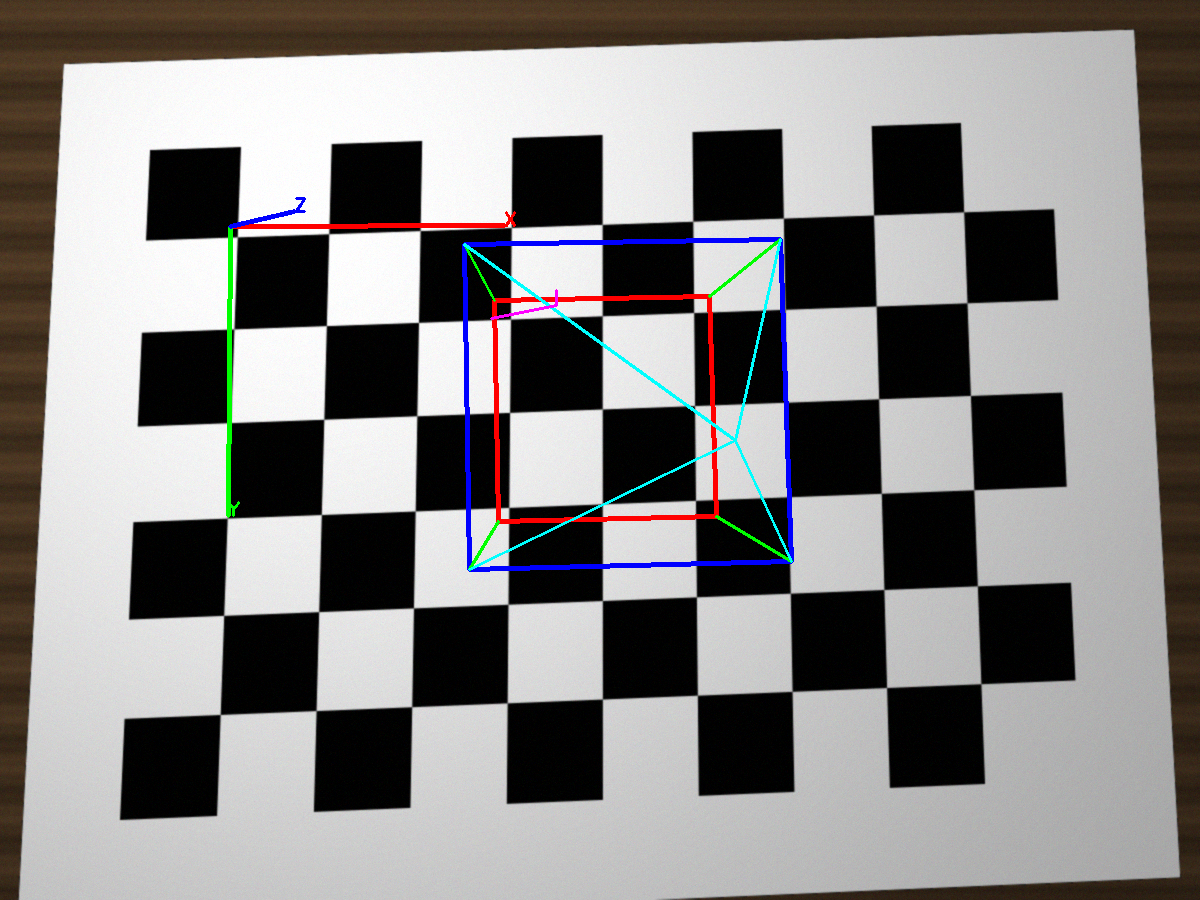
\includegraphics[width=\textwidth]{data/ar_output/ar_frame_1.png}
        \caption{AR Overlay: Frame 1}
    \end{subfigure}
    \hfill
    \begin{subfigure}[b]{0.48\textwidth}
        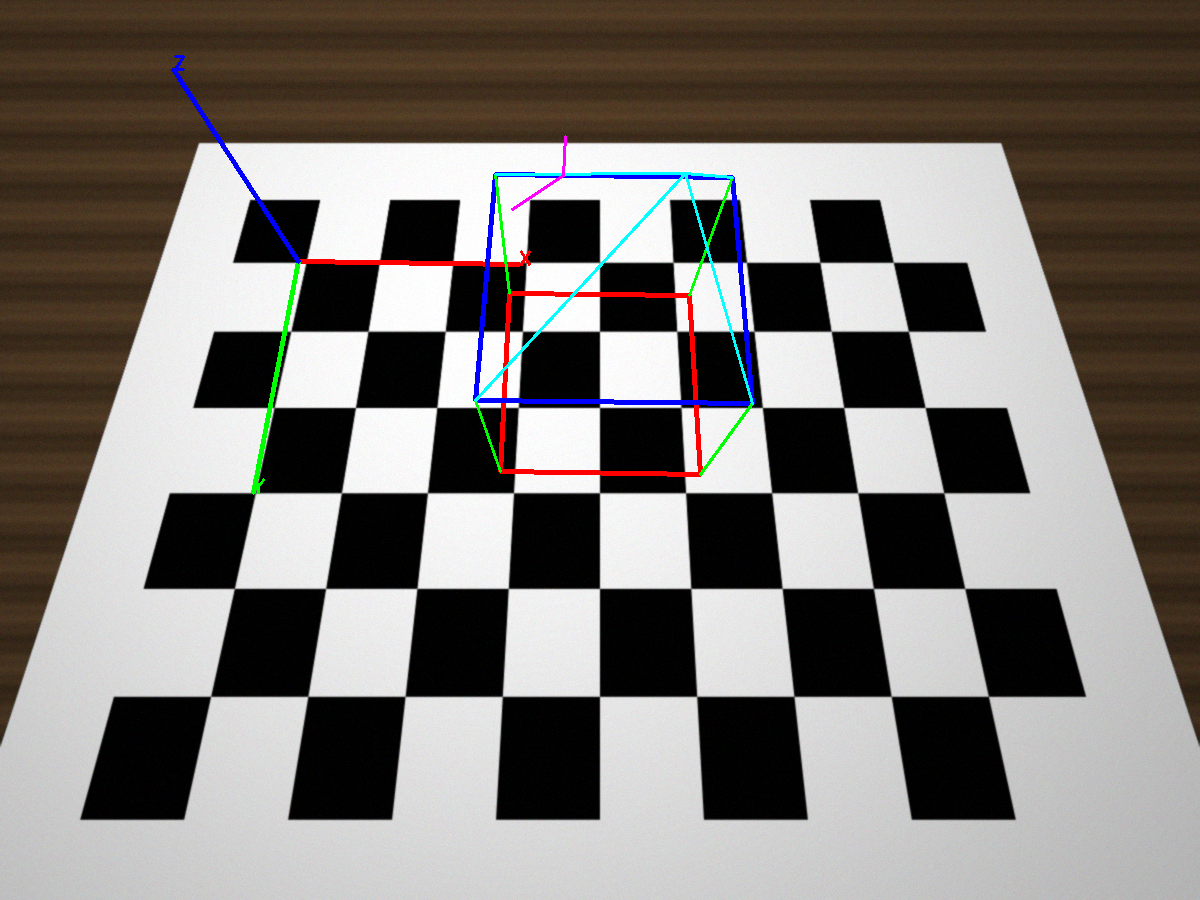
\includegraphics[width=\textwidth]{data/ar_output/ar_frame_3.png}
        \caption{AR Overlay: Frame 3}
    \end{subfigure}
    \caption{Visual overlays representing 3D coordinate axes and a custom 3D house virtual object drawn on top of the checkerboard.}
    \label{fig:ar_overlay}
\end{figure}

%------------------------------------------------------------
\subsection*{Task 7: Robust Feature Detection}
%------------------------------------------------------------

I created a separate program to extract robust features from a video stream. It supports two modes: Harris corners and ORB keypoints. The user can toggle between modes using trackbars or keypresses.

The Harris corner detector computes the structure tensor at each pixel. It uses a Sobel filter of size 3 and a block size of 3. It calculates a corner response score based on the eigenvalues of the tensor. ORB uses the FAST algorithm to locate keypoints and BRIEF to compute binary descriptors. Changing the threshold values alters the sensitivity. Higher thresholds reduce noise but miss weaker corners.

Figure~\ref{fig:features} shows the Harris corner detections and the ORB keypoints on the target.

\begin{figure}[H]
    \centering
    \begin{subfigure}[b]{0.48\textwidth}
        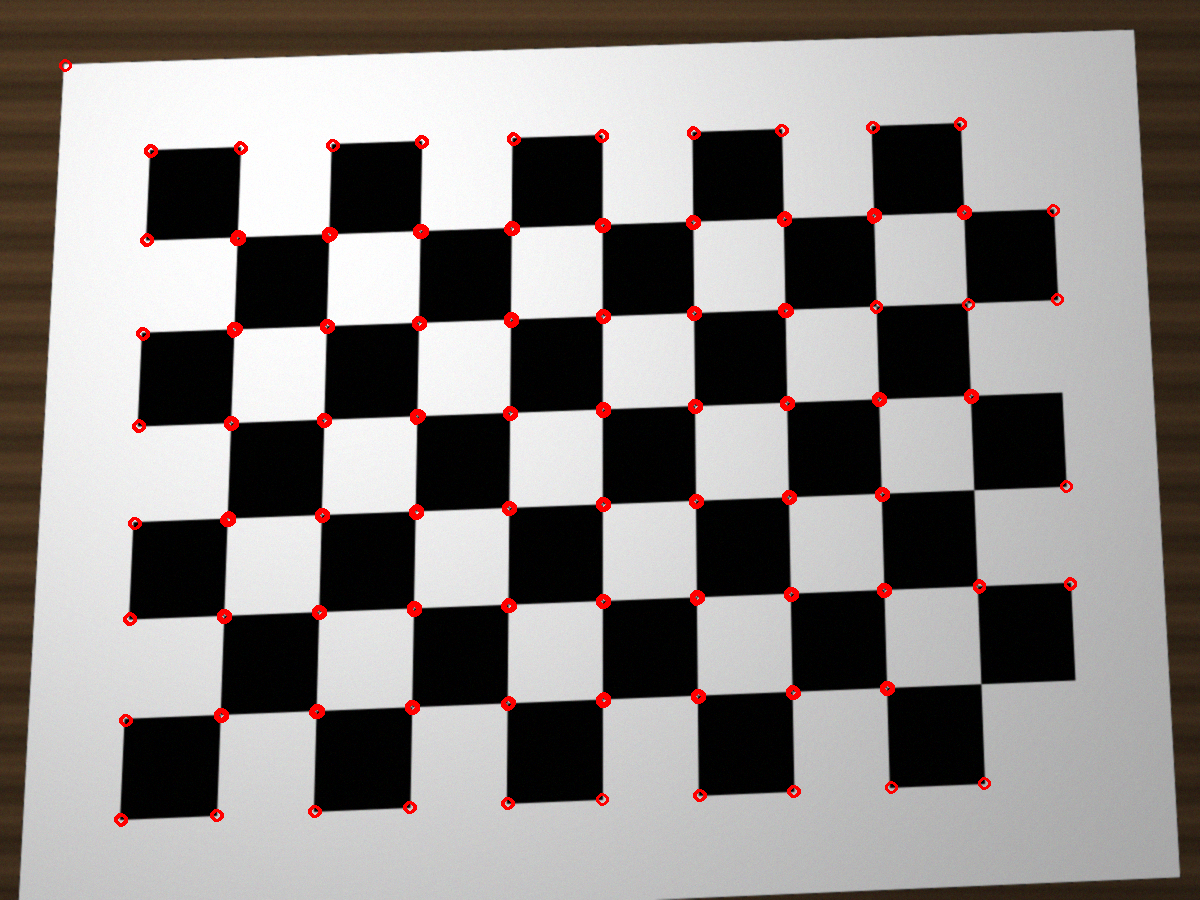
\includegraphics[width=\textwidth]{data/ar_output/features_harris_frame_1.png}
        \caption{Harris Corners}
    \end{subfigure}
    \hfill
    \begin{subfigure}[b]{0.48\textwidth}
        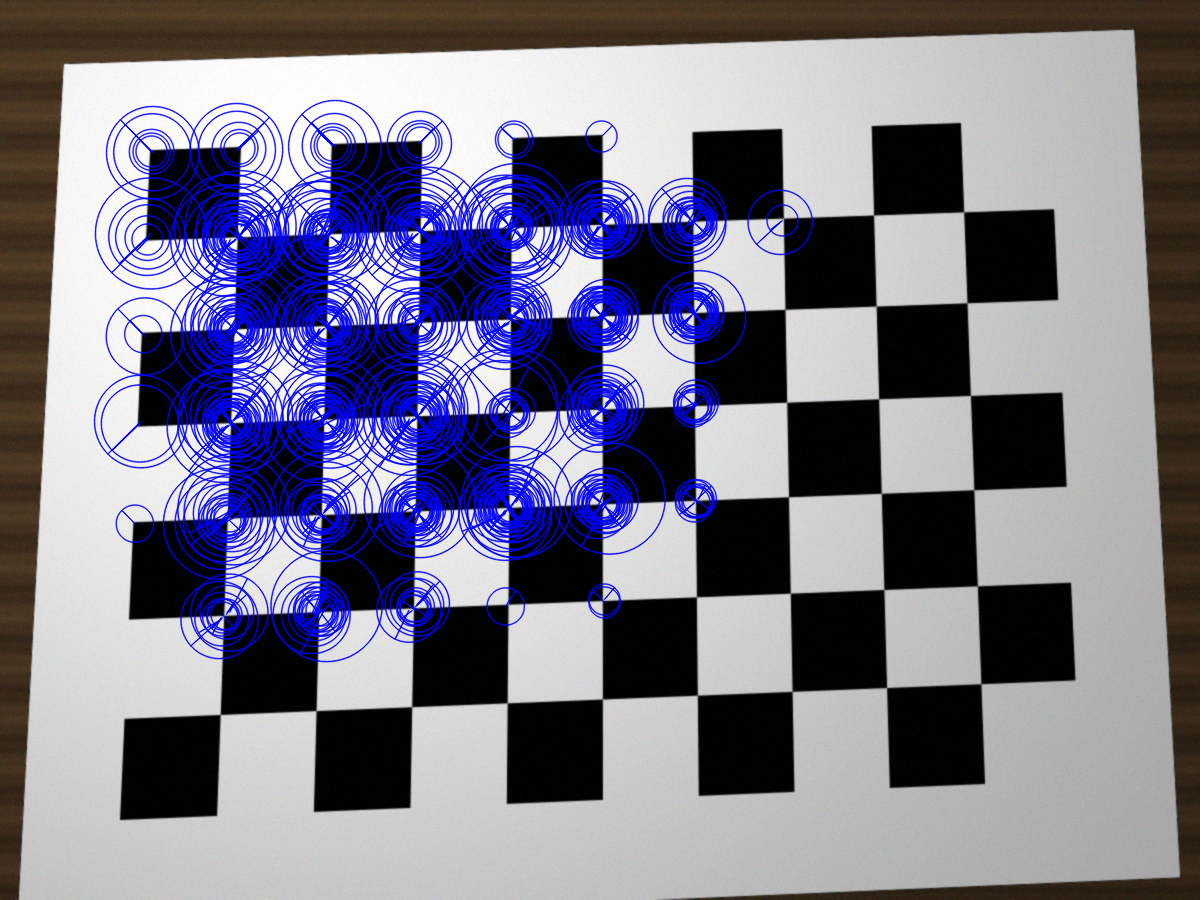
\includegraphics[width=\textwidth]{data/ar_output/features_orb_frame_1.png}
        \caption{ORB Keypoints}
    \end{subfigure}
    \caption{Robust feature maps detected on the calibration target.}
    \label{fig:features}
\end{figure}

These local feature points can serve as the basis for markerless AR. By matching ORB or SIFT descriptors between a reference image and a live video frame, we can establish 2D-to-2D matches. Using RANSAC, we can find the homography or relative pose without needing a structured checkerboard target. This allows placing virtual objects on any flat surface or picture.

% ============================================================
\section*{Reflection}
% ============================================================

This project helped me understand the geometry behind camera calibration and pose estimation. Working with perspective projection in C++ made the theory of camera matrices and lens distortion very clear.

Setting up the coordinate axes correctly was challenging at first. I learned that defining the 3D points on the board plane with negative Y values ensures the Z-axis projects towards the camera. If I used positive Y values, the Z-axis would point away from the viewer. This would make rendering 3D objects confusing.

I also learned how lens distortion affects image coordinates. Radial and tangential distortion alter the positions of pixels. Estimating five distortion parameters corrects these errors. This optimization step makes the 3D virtual house align perfectly with the target grid. 

Finally, I realized the difference between marker-based and markerless tracking. The chessboard target is easy to detect because of its high-contrast corners. However, it is not practical for real AR applications. Using local feature detectors like ORB and Harris corners is much more flexible. It shows how computer vision can align virtual content with any textured surface. This was a valuable hands-on experience in combining geometry and software engineering.

% ============================================================
\section*{Acknowledgements}
% ============================================================

\begin{itemize}
    \item OpenCV Documentation (\url{https://docs.opencv.org/}) for calibration, pose solving, and projection tutorials.
    \item I completed this project individually.
    \item AI was used for debugging and code structure assistance.
\end{itemize}

\end{document}
